%Round Bottome Flask
\documentclass[preview]{standalone}
\usepackage{tikz}
\usetikzlibrary{calc}

\begin{document}
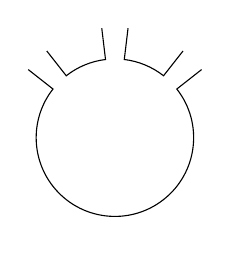
\begin{tikzpicture}
	\pgfmathsetmacro{\R}{1}				%radius of flask
	\pgfmathsetmacro{\neck}{3}			%number of necks
	\pgfmathsetmacro{\pos}{90}			%position of first neck in degrees
	\pgfmathsetmacro{\ang}{45}			%separation of necks in degrees
	\pgfmathsetmacro{\taperwidth}{24}	%Width of the joint taper
	\pgfmathsetmacro{\taperlength}{40}	%Length of the joint taper

	%calculated
	\pgfmathsetmacro{\firstangle}{\pos-\ang}	%Calculating the far right angle
	\pgfmathsetmacro{\secondangle}{\pos+\ang}	%Calculating the far left angle

	%clockwise from 90
	\coordinate (a) at ({\pos-atan((\taperwidth/200)/\R)}:\R+\taperlength/100) [fill=none]{};
	\coordinate (b) at ({\pos-atan((\taperwidth/200)/\R)}:\R) [fill=none]{};
	\coordinate (c) at ({\firstangle+atan((\taperwidth/200)/\R)}:\R) {};
	\coordinate (d) at ({\firstangle+atan((\taperwidth/200)/\R)}:\R+\taperlength/100) {};
	\coordinate (e) at ({\firstangle-atan((\taperwidth/200)/\R)}:\R+\taperlength/100) {};
	\coordinate (f) at ({\firstangle-atan((\taperwidth/200)/\R)}:\R) {};
	\coordinate (g) at ({\secondangle+atan((\taperwidth/200)/\R)}:\R) {};
	\coordinate (h) at ({\secondangle+atan((\taperwidth/200)/\R)}:\R+\taperlength/100) {};
	\coordinate (i) at ({\secondangle-atan((\taperwidth/200)/\R)}:\R+\taperlength/100) {};
	\coordinate (j) at ({\secondangle-atan((\taperwidth/200)/\R)}:\R) {};
	\coordinate (k) at ({\pos+atan((\taperwidth/200)/\R)}:\R) {};
	\coordinate (l) at ({\pos+atan((\taperwidth/200)/\R)}:\R+\taperlength/100) {};

	\draw (a) -- (b) arc ({\pos-atan((\taperwidth/200)/\R)}:{\firstangle+atan((\taperwidth/200)/\R)}:\R) -- (d);
	\draw (e) -- (f) arc ({\firstangle-atan((\taperwidth/200)/\R)}:{\secondangle+atan((\taperwidth/200)/\R)-360}:\R) -- (h);
	\draw (i) -- (j) arc ({\secondangle-atan((\taperwidth/200)/\R)}:{\pos+atan((\taperwidth/200)/\R)}:\R) -- (l);
\end{tikzpicture}
\end{document}
